% Options for packages loaded elsewhere
\PassOptionsToPackage{unicode}{hyperref}
\PassOptionsToPackage{hyphens}{url}
%
\documentclass[
]{article}
\usepackage{amsmath,amssymb}
\usepackage{lmodern}
\usepackage{ifxetex,ifluatex}
\ifnum 0\ifxetex 1\fi\ifluatex 1\fi=0 % if pdftex
  \usepackage[T1]{fontenc}
  \usepackage[utf8]{inputenc}
  \usepackage{textcomp} % provide euro and other symbols
\else % if luatex or xetex
  \usepackage{unicode-math}
  \defaultfontfeatures{Scale=MatchLowercase}
  \defaultfontfeatures[\rmfamily]{Ligatures=TeX,Scale=1}
\fi
% Use upquote if available, for straight quotes in verbatim environments
\IfFileExists{upquote.sty}{\usepackage{upquote}}{}
\IfFileExists{microtype.sty}{% use microtype if available
  \usepackage[]{microtype}
  \UseMicrotypeSet[protrusion]{basicmath} % disable protrusion for tt fonts
}{}
\makeatletter
\@ifundefined{KOMAClassName}{% if non-KOMA class
  \IfFileExists{parskip.sty}{%
    \usepackage{parskip}
  }{% else
    \setlength{\parindent}{0pt}
    \setlength{\parskip}{6pt plus 2pt minus 1pt}}
}{% if KOMA class
  \KOMAoptions{parskip=half}}
\makeatother
\usepackage{xcolor}
\IfFileExists{xurl.sty}{\usepackage{xurl}}{} % add URL line breaks if available
\IfFileExists{bookmark.sty}{\usepackage{bookmark}}{\usepackage{hyperref}}
\hypersetup{
  pdftitle={Criminalization of Girls in California: A Fact Sheet},
  pdfauthor={Shaina Mackin \textbar{} The Vera Institute},
  hidelinks,
  pdfcreator={LaTeX via pandoc}}
\urlstyle{same} % disable monospaced font for URLs
\usepackage[margin=1in]{geometry}
\usepackage{graphicx}
\makeatletter
\def\maxwidth{\ifdim\Gin@nat@width>\linewidth\linewidth\else\Gin@nat@width\fi}
\def\maxheight{\ifdim\Gin@nat@height>\textheight\textheight\else\Gin@nat@height\fi}
\makeatother
% Scale images if necessary, so that they will not overflow the page
% margins by default, and it is still possible to overwrite the defaults
% using explicit options in \includegraphics[width, height, ...]{}
\setkeys{Gin}{width=\maxwidth,height=\maxheight,keepaspectratio}
% Set default figure placement to htbp
\makeatletter
\def\fps@figure{htbp}
\makeatother
\setlength{\emergencystretch}{3em} % prevent overfull lines
\providecommand{\tightlist}{%
  \setlength{\itemsep}{0pt}\setlength{\parskip}{0pt}}
\setcounter{secnumdepth}{-\maxdimen} % remove section numbering
\ifluatex
  \usepackage{selnolig}  % disable illegal ligatures
\fi

\title{Criminalization of Girls in California: A Fact Sheet}
\author{Shaina Mackin \textbar{} The Vera Institute}
\date{March 29, 2022}

\begin{document}
\maketitle

\hypertarget{california-is-one-of-the-united-states-top-incarcerators-of-girls} of detentions between 2012-2017 were in secure
facilities.

\hypertarget{top-incarcerating-counties}{%
\subsection{Top Incarcerating
Counties}\label{top-incarcerating-counties}}

\begin{verbatim}
Counties that detained the most girls in 2017:           Counties most likely to detain girls in 2017:
\end{verbatim}

\begin{table}

\begin{tabular}[t]{l|l|r}
\hline
County & Percent of State Total & Number Detained\\
\hline
Los Angeles & 12.5\% & 577\\
\hline
San Bernadino & 10.99\% & 509\\
\hline
Ventura & 7.12\% & 330\\
\hline
Orange & 6.54\% & 303\\
\hline
Contra Costa & 5.12\% & 237\\
\hline
Santa Clara & 4.62\% & 214\\
\hline
Santa Barbara & 4.23\% & 196\\
\hline
Kern & 3.97\% & 184\\
\hline
Fresno & 3.5\% & 162\\
\hline
Mendocino & 3.3\% & 153\\
\hline
\end{tabular}
\begin{tabular}[t]{l|l|r}
\hline
County & Percent of Cases & Number of Times in Top 10\\
\hline
Glenn & 100\% & 6\\
\hline
Modoc & 100\% & 4\\
\hline
Mendocino & 56.7\% & 5\\
\hline
Sonoma & 49.2\% & 2\\
\hline
Imperial & 48.7\% & 4\\
\hline
San Francisco & 48.4\% & 3\\
\hline
Shasta & 47.8\% & 5\\
\hline
Ventura & 43.5\% & 2\\
\hline
Santa Clara & 41.6\% & 2\\
\hline
San Luis Obispo & 41.1\% & NA\\
\hline
\end{tabular}
\end{table}

\hypertarget{average-daily-populations}{%
\subsection{Average Daily Populations}\label{average-daily-populations}}

California's Board of State and Community Corrections (BSCC) reports
Average Daily Populations (ADP) of juvenile facilities by county. In
2021, Los Angeles County's annual sum of monthly ADPs was over twice
that of Kern's, the second highest.

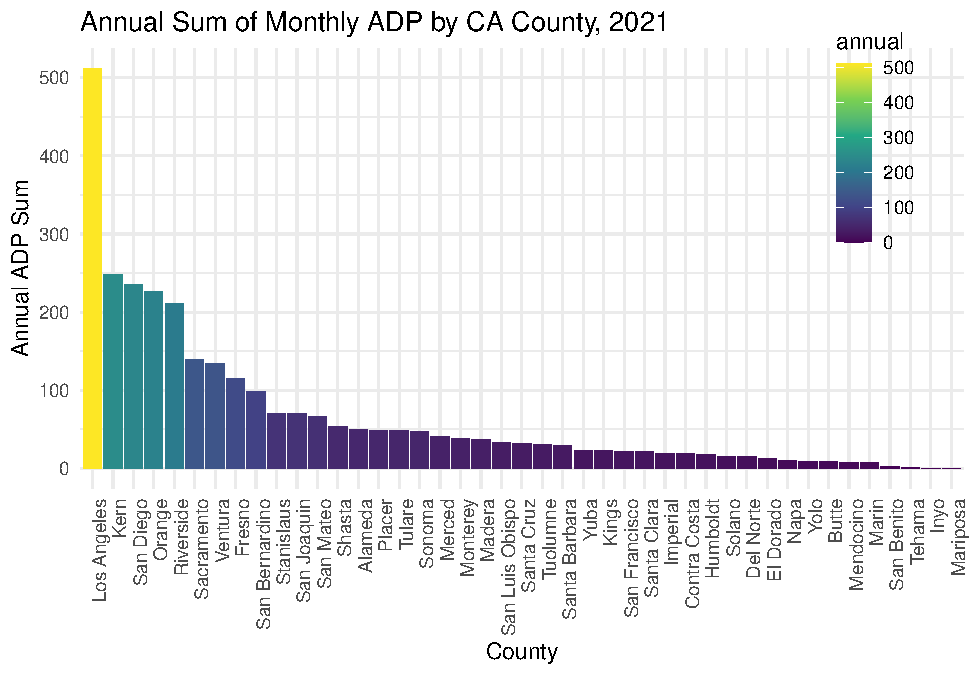
\includegraphics{ADP_files/figure-latex/annual_adp-1.pdf}

\hypertarget{zooming-in-on-santa-clara-county} decrease (n=\textbf{3}).

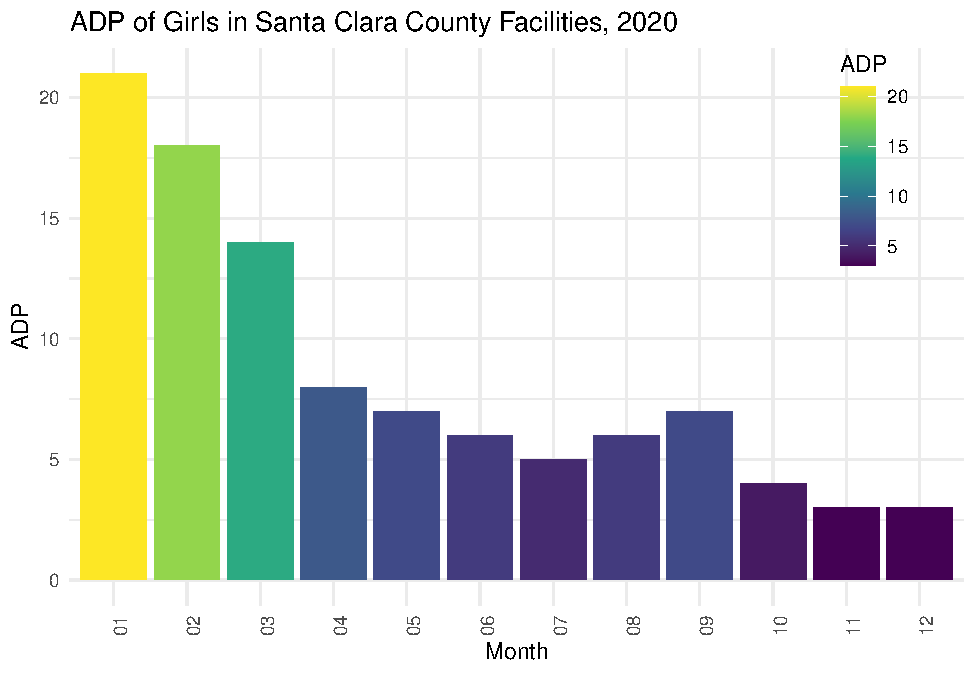
\includegraphics{ADP_files/figure-latex/santa_clara_county-1.pdf}

\end{document}
